\chapter{Architettura del progetto}

\section{Demo starter}
Come input alla realizzazione della nostra applicazione, siamo partiti da una demo offerta direttamente da MediaPipe. In questa applicazione viene data la possibilità all'utente di visualizzare la mappatura delle proprie mani scegliendo diverse modalità di acquisizione dell'immagine.
Oltre a file ausiliari come il \textit{manifest} o gli \textit{xml} di configurazione, il cuore del progetto è rappresentato da 3 file nel package \texttt{hands/ja-} \texttt{va/com/google/mediapipe/examples/hands}.
\begin{figure}[H]
    \centering
    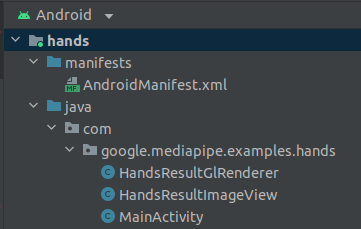
\includegraphics[width=0.5\textwidth]{images/struct_demo.png}
\end{figure}
\noindent Ovviamente, \texttt{MainActivity} corrisponde all'entry point dell'applicazione ed eredita infatti da \texttt{AppCompatActivity}.\\
\\
\noindent Nonostante noi ci siamo concentrati solo sull'input da streaming video, l'applicazione mette a disposizione 3 diverse modalità di acquisizione dell'input, rappresentate dall'enumerativo \texttt{InputSource} all'interno del quale troviamo \texttt{CAMERA}, \texttt{VIDEO} e \texttt{IMAGE}.\\


\section{Struttura del progetto}
\begin{figure}[H]
    \centering
    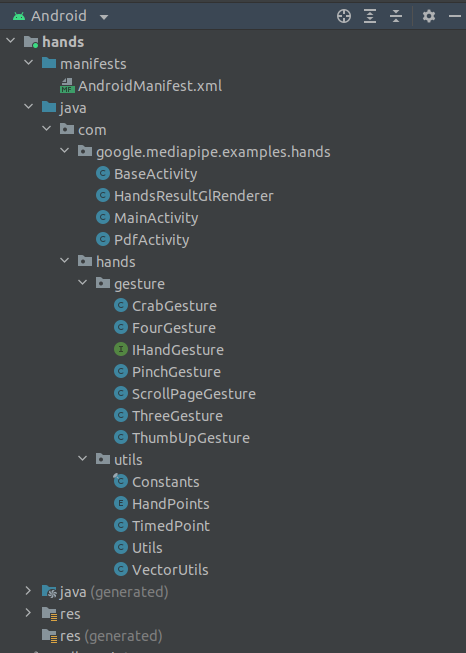
\includegraphics[width=0.8\textwidth]{images/struct_progetto.png}
\end{figure}
All'interno del package \texttt{hands/java/com/google/mediapipe/examples/hands} abbiamo potuto eliminare la classe \texttt{HandsResultImageView}, utile solo con acquisizione dell'input tramite immagine statica; mentre la classe \texttt{HandsResultGlRenderer}, per il rendering su schermo, è stata lasciata sostanzialmente inalterata.\\
Sono state invece applicate delle modifiche consistenti alla classe \texttt{MainActivity} (aggiungendo anche altre due classi \textit{Activity}) per implementare la logica applicativa.\\


\subsection{BaseActivity, MainActivity e PdfActivity}
Mentre prima era \texttt{MainActivity} ad ereditare da \texttt{AppCompatActivity}, ora questo avviene per \texttt{BaseActivity}, da cui erediteranno poi la classe \texttt{PdfActivity} e la nuova \texttt{MainActivity}.\\
Abbiamo scelto di adottare questa strategia implementativa per suddividere in modo chiaro e pulito le funzionalità esposte dalle due classi:
\begin{itemize}
    \item \texttt{MainActivity}: si occupa di definire il layout dell'applicazione nel caso in cui si voglia visualizzare su tutto lo schermo la propria mano, con alcune \texttt{TextView} per mostrare il riconoscimento di determinate \textbf{gesture}.
    \item \texttt{PdfActivity}: corrisponde al cuore dell'applicazione, definendo un layout nel quale è presente un file \texttt{pdf} da leggere ed una piccola vista della fotocamera interna dello smartphone. Quest'ultima ha lo scopo di mostrare all'utente il movimento della propria mano, tramite la quale avrà la possibilità di interagire con il file.
\end{itemize}
\noindent Entrambe le \textit{activities} hanno quindi lo scopo di mostrare la mano ed il riconoscimento di gesture, la prima \textit{"loggando"} l'eventuale riconoscimento, la seconda interagendo con il pdf.\\
Per fare questo, all'interno di ognuna, viene definito un \textbf{listener} che controlla continuamente l'eventuale associazione di un movimento della mano ad una gesture. Sono state infatti create 6 classi, una per gesture, che si occupano di effettuare il controllo sulla base dei \textbf{landmarks} passati in input dalle \textit{activities}.\\
\\
Prima di concentrarci su queste classi, di seguito vengono esposte caratteristiche più dettagliate di ognuna delle \textit{activitites} presentate sopra.

\subsubsection{BaseActivity}
Questa classe funge da contenitore per tutte quelle variabili e funzioni comuni sia a \texttt{MainActivity} sia a \texttt{PdfActivity} (perciò dichiarate con la clausola \texttt{protected}). Questa permette di evitare la ridondanza di codice.\\

\paragraph{Variabili} Alcune delle variabili comuni definite sono:
\begin{itemize}
    \item \texttt{Hands}, tramite la quale viene recuperato il \textbf{listener} nominato sopra, da cui poi otteniamo i risultati del mapping effettuato dalla pipeline di riconoscimento di MediaPipe.
    \item \texttt{InputSource}, che rappresenta la modalità di acquisizione dell'immagine (da noi sarà sempre \texttt{CAMERA}).
    \item \texttt{CameraInput}, che rappresenta la ricezione dell'input dalla fotocamera.
\end{itemize}
\noindent Abbiamo poi \texttt{SolutionGlSurfaceView$<$HandsResult$>$} e \texttt{HandsResultGlRenderer} per la definizione del layout e per il rendering.\\ 
Infine, sono presenti le istanze di tutte quelle classi che effettuano il rilevamento delle gesture, che, come detto in precedenza, sono necessarie ad entrambe le \texttt{activities}, anche se con scopi diversi.

\paragraph{Metodi} Essendo che questa classe eredita da \texttt{AppCompatActivity}, è necessario effettuare l'\texttt{override} dei seguenti metodi:
\begin{itemize}
    \item \texttt{onCreate}, accetta un \texttt{Bundle} in input, utilizzato per chiamare la \texttt{onCreate} della classe estesa. In Android Studio i \textit{Bundle} si utilizzano solitamente per il passaggio di dati da un attività all'altra: in questo caso abbiamo un istanza di uno stato salvato precedentemente (e.g. l'applicazione era stata messa in background). All'interno di questa funzione è solito definire il layout della pagina, ma abbiamo scelto di farlo solo nelle \textit{activities specializzate} che erediteranno da \texttt{BaseActivity}.
    \item \texttt{onPause}, nella quale viene chiamata la \texttt{onPause} della classe estesa per poi nascondere la visibilità del layout (\texttt{glSurfaceView}) e fermare infine il flusso video in input dalla fotocamera.
    \item \texttt{onResume}, dove dopo essere stata chiamata la \texttt{onResume} della classe estesa, si istanzia un nuovo \texttt{CameraInput} (passandogli l'\textit{activity} corrente) per poi settare un nuovo \textit{FrameListener}. Successivamente viene utilizzata l'istanza di \texttt{SolutionGlSurfaceView<HandsResult>} per chiamare il metodo interno \texttt{post}, passandogli la funzione interna \texttt{startCamera()} (il cui scopo è quello di inizializzare lo streaming video). In questo modo, tramite la \texttt{post} ereditata dalla classe \texttt{View}, viene eseguita la funzione passata ed esposto l'output nell' interfaccia utente.
\end{itemize}
\noindent Sono presenti poi ulteriori funzioni che vengono utilizzate da \texttt{MainActivity} e \\\texttt{PdfActivity} per inizializzare la pipeline di acquisizione dell'input e per terminarla. Verranno analizzate in seguito.


\newpage
\subsubsection{MainActivity}
Abbiamo detto che lo scopo di questa \textit{activity} è quello di mostrare su schermo l'eventuale riconoscimento di determinate gesture. Perciò, oltre alle variabili definite nella classe estesa, le uniche variabili globali presenti sono una serie \texttt{TextView}, una per ogni gesture.\\
Viene effettuato l'\texttt{override} delle funzioni ereditate da \texttt{AppCompatActivity} e, mentre \texttt{onPause} e \texttt{onResume} chiamano solamente le relative funzioni della classe \texttt{BaseActivity}, la \texttt{onCreate} si occupa inoltre di \underline{inizializzare lo streaming video} e di definire il layout della pagina, istanziando anche un nuovo bottone per accedere alla funzionalità di interazione coi file \texttt{pdf}.\\
\\
Per quanto riguarda l'inizializzazione dello streaming video, vengono utilizzate due funzioni:
\begin{itemize}
    \item \texttt{setupLiveDemoUiComponents}, all'interno della quale viene definito un bottone per attivare lo streaming che, una volta cliccato, causerà la chiamata alla stessa funzione della classe estesa (il cui scopo è quello di fermare la pipeline di acquisizione attuale (nel caso in cui la modalità di acquisizione sia diversa da \texttt{CAMERA})). Successivamente, viene chiamata la funzione che implementa effettivamente la pipeline, mostrata qui sotto.
    \item \texttt{setupStreamingModePipeline}, questa funzione è divisa sostanzialmente in 3 parti, oltre ad una preliminare nella quale vengono inizializzate le \texttt{TextView}. \begin{enumerate}
        \item chiamata alla funzione \texttt{firstSetupStreamingModePipeline} di \texttt{BaseActivity} che crea delle nuove istanze di \texttt{HandsResultGlRenderer}, \texttt{Hands} e \texttt{glSurfaceView}. Tramite essa inizia lo streaming dalla fotocamera e, concorrentemente, la pipeline per il mapping dei \textbf{landmarks} della mano.
        \item settato il \textbf{listener} per il riconoscimento delle gesture, all'interno del quale vengono effettuate delle chiamate alle classi per il controllo e mostrato l'eventuale riconoscimento colorando le \texttt{Textview} definite prima.
        \item chiamata alla funzione \texttt{lastSetupStreamingModePipeline} di \texttt{BaseActivity} che chiama il metodo \texttt{post} di \texttt{glSurfaceView} visto in precedenza e definisce il nuovo \texttt{FrameLayout} con i dati trovati nella fase precedente.
    \end{enumerate}
\end{itemize}


\subsubsection{PdfActivity}
Il funzionamento di questa classe è analogo a quella mostrata in precedenza. Viene ovviamente differenziato il layout della pagina e, all'interno del \textit{listener} della funzione \texttt{setupStreamingModePipeline}, vengono associate le varie gesture riconosciute ad azioni che permettono di interagire con il file \texttt{pdf} che si sta visualizzando.


\subsection{Gesture}
All'interno del package \texttt{hands/java/com/hands/gesture} sono presenti 6 classi, una per ogni gesture, ed una interfaccia (\texttt{IHandGesture}).\\
Quest'ultima dichiara la funzione che tutte le altri classi, tranne \texttt{ScrollPageGesture}, implementeranno per effettuare il controllo delle gesture.
\begin{center}
    \begin{minted}[bgcolor=lightgray,framesep=2mm,baselinestretch=1.2,fontsize=\footnotesize,escapeinside=||,mathescape=true]{java}
        boolean checkGesture(HandsResult handsResult);
    \end{minted}
\end{center}
\noindent \texttt{ScrollPageGesture} non implementa l'interfaccia in quanto la sua funzione di controllo restituisce un intero.\\
\\
\noindent La logica all'interno delle funzioni di controllo verrà analizzata nei capitoli successivi.

\subsection{Utils}
All'interno del package \texttt{hands/java/com/hands/utils} sono presenti 5 classi di utilità.\\
\subsubsection{TimedPoint}
Rappresenta un oggetto composto dalle seguenti proprietà.
\begin{minted}[bgcolor=lightgray,framesep=2mm,baselinestretch=1.2,fontsize=\footnotesize,escapeinside=||,mathescape=true]{java}
    public class TimedPoint {

        public float x;
        public float y;
        public long timestamp;
        ...
    }
\end{minted}

\noindent Viene utilizzata all'interno di \texttt{ScrollPageGesture} per calcolare la velocità di movimento tra due landmarks.\\
Viene usato il \textit{timestamp} per calcolare il tempo trascorso e le coordinate per la distanza, da cui si ricava appunto la velocità.

\newpage
\subsubsection{HandPoints}
Classe di tipo enumerativo per associare delle costanti letterali ai 21 punti che rappresentano i landmarks forniti da \texttt{MediaPipe}.
\begin{minted}[bgcolor=lightgray,framesep=2mm,baselinestretch=1.2,fontsize=\footnotesize,escapeinside=||,mathescape=true]{java}
    public enum HandPoints {
        WRIST(0),
        THUMB_BASE(1),
        THUMB_LOWER(2),
        THUMB_UPPER(3),
        THUMB_TIP(4),
        ...
    }
\end{minted}

\subsubsection{Constants}
Sono presenti alcune costanti di utilità.
\begin{minted}[bgcolor=lightgray,framesep=2mm,baselinestretch=1.2,fontsize=\footnotesize,escapeinside=||,mathescape=true]{java}
    public final class Constants {

        public static final int NUMERO_LIVELLI = 70;
        ...
    }
\end{minted}

\subsubsection{Utils e VectorUtils}
All'interno di queste due classi sono presenti funzioni utilizzate dalle classi per il controllo delle gesture.\\
In ognuna delle classi ci sono funzioni di basso livello che effettuano i calcoli di base, come ad esempio la distanza tra due punti. Per motivi di efficienza, abbiamo scelto di implementarle con delle chiamate a codice \texttt{C} (analisi nella \hyperref[chap:cpp]{\underline{sezione successiva}}).\\
\\
\noindent Abbiamo poi altre funzioni di più alto livello, come \texttt{fingerLevelsToWrist()}, che utilizzano le funzioni di base citate sopra per elaborare i dati, offrendo alle classi che le chiamano un interfaccia semplice e comoda da usare.

\newpage
\subsection{Binding funzioni C++}
\label{chap:cpp}
\noindent
Molte delle funzionalità che abbiamo implementato richiedono una quantità moderatamente elevata di calcoli, che diventa estremamente rilevante se si considera che questi calcoli vengono eseguiti circa 30 volte al secondo, abbiamo quindi deciso di implementare alcune funzioni chiave in C++ per ottenere performance più adeguate.\\

\noindent
Avvalendoci della JNI (Java Native Interface) abbiamo potuto implementare funzioni in C++ e poi richiamarle dal nostro codice Java.\\

\noindent
Un semplice esempio di una funzione che abbiamo implementato in \texttt{C++} utilizzando la JNI:
\begin{minted}[bgcolor=lightgray,framesep=2mm,baselinestretch=1.2,fontsize=\footnotesize,escapeinside=||,mathescape=true]{cpp}
extern "C" JNIEXPORT jdouble JNICALL
Java_com_hands_utils_VectorUtils_dotProductWrap(JNIEnv *env, jclass clazz,
                                                jdoubleArray v1,
                                                jdoubleArray v2) {
    //return dot product of v1 and v2
    jdouble *v1Array = env->GetDoubleArrayElements(v1, nullptr);
    jdouble *v2Array = env->GetDoubleArrayElements(v2, nullptr);
    jsize v1Length = env->GetArrayLength(v1);
    jsize v2Length = env->GetArrayLength(v2);
    jdouble result = 0;
    if (v1Length == v2Length) {
        for (int i = 0; i < v1Length; i++) {
            result += v1Array[i] * v2Array[i];
        }
    }
    return result;
}
\end{minted}

\noindent Molte delle funzioni nelle classi \texttt{VectorUtils} e \texttt{Utils} sono state implementate in questo modo dato che contengono la maggior parte delle funzionalità matematiche utilizzate.\\
Tuttavia l'incremento ottenuto utilizzando questa tecnica, anche se rilevante, non è stato quello sperato. La causa potrebbe risiedere nell'overhead introdotto da ogni singola chiamata alla libreria \texttt{C++} dinamica creata.

